%slide di introduzione ai fondamenti degli schemi xml
% [+]leggere capitolo due "XML Schema Languages" del libro Advanced XML Applications from the Experts at The XML Guild
% Only TYPED xml can be validated with an XML schema
% When XML documents need to follow a certain structure and the values of attributes and elements need to follow a set of rules
% A method to describe the XML structure 
% A method to validate the XML data
%  get a clear idea about the required XML structure from the schema.
% Since a schema explains the required XML structure much better than a word document or a document of any other kind, there are no chances of misunderstanding or misinterpreting what is required.
% Validation of the XML data submitted by the client applications became easier.
%  define the validation rules.
%  list of validations that had to be included in the Schema

% XML Schema provides a kind of document grammar, naming the possible components and constraining the organization of an document. 
% XML Schema makes it possible to express constraints
% The Rules can be easly checked by an automatic processor: a validator

% An XML schema describes and validates XML documents.

% Should this piece of data go in an element or in an attribute? On many occasions, your piece of data could be stored equally well in an attribute as in an element with no loss of information. It is being largely a matter of personal taste



% For different users to share a vocabulary effectively, rules must be developed that
% specifically control what code and content a document from that vocabulary might
% contain. This is done by attaching either a Document Type Definition (DTD) or a
% schema to the XML document containing the data. Both DTDs and schemas contain
% rules for how data in a document vocabulary should be structured. A DTD defines the
% structure of the data and, very broadly, the types of data allowable. A schema more
% precisely defines the structure of the data and specific data restrictions.

% If an XML document is part of a vocabulary with a defined DTD or schema, it also
% must be tested to ensure that it satisfies the rules of that vocabulary. A well-formed XML
% document that satisfies the rules of a DTD or schema is said to be a valid document.

% frame 02
\begin{frame}
    \frametitle{Elementi per la definizione degli schemi xml}
    \framesubtitle{principi}
    \addtocounter{nframe}{1}

    we need to make sure that the data that we receive follows a certain XML structure and should contain values which are coherent. 

    Your function needs to make sure that the caller passes correct XML data. You could make use of an XML Schema to perform this validation.

    Performing such validations without the help of a SCHEMA will be extremely difficult most of the time.


\end{frame}

% frame 03
\begin{frame}
    \frametitle{Elementi per la definizione degli schemi xml}
    \framesubtitle{principi}
    \addtocounter{nframe}{1}

    Make sure that the XML document is structured exactly the way your function expects it to be.

   We need an XML schema when we need to make sure that the XML document that we need to work with is in the expected format.
   Make sure that the values of elements and attributes are within the accepted range.

   When data is managed and exchanged in XML format, there needs to be clear agreement about the structure of the XML document.

   There needs to be a contract between the caller and the callee about the XML document being exchanged.

   validate the XML document to make sure that it adheres to the format defined in the contract.


\end{frame}



% frame 04
\begin{frame}
    \frametitle{Elementi per la definizione degli schemi xml}
    \framesubtitle{principi}
    \addtocounter{nframe}{1}

    A Schema provides such the contract. 
    \\ It defines the structure of the XML document. 
    \\ It defines rules to validate the value of elements and attributes as well as their formats. 
    \\ Once a schema is defined, a Schema Validator can validate an XML document against the rules defined in the Schema.


\end{frame}


% frame 05
\begin{frame}
    \frametitle{Elementi per la definizione degli schemi xml}
    \framesubtitle{Tipi di formalismi per definire schemi XML}
    \addtocounter{nframe}{1}

   DTD, XDR, SOX, Schematron, DSD, DCD, DDML, RELAX NG

\end{frame}

\subsection{DTD}
%slide di introduzione ai fondamenti di Document Type Definition

%frame 01
\begin{frame}
    \frametitle{Elementi per la definizione degli schemi xml}
    \framesubtitle{Principi Document Type Definition}
    \addtocounter{nframe}{1}

    \begin{block}{Esempio DTD}
        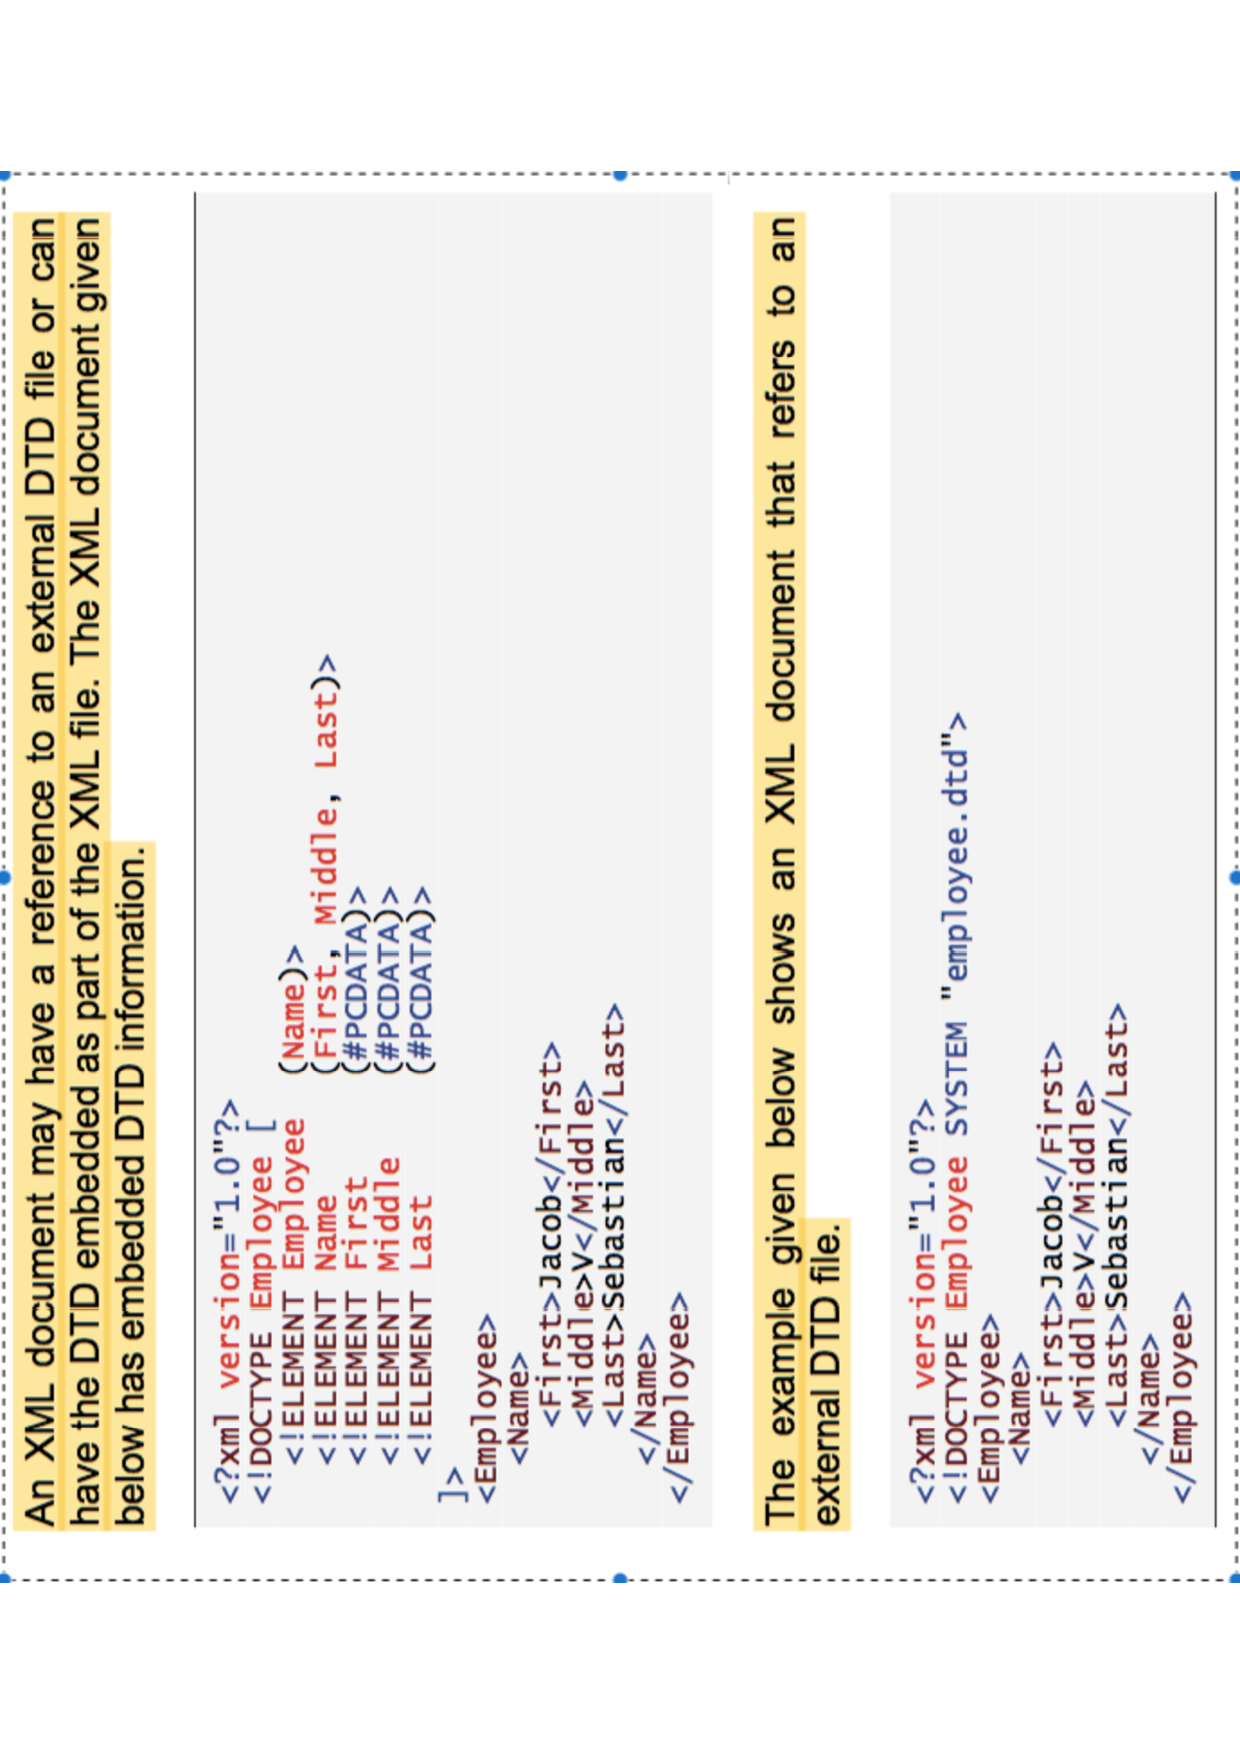
\includegraphics[width=.5\textwidth]{imgs/dtd_1.pdf}
    \end{block}

\end{frame}


\begin{frame}
    \frametitle{Elementi per la definizione degli schemi xml}
    \framesubtitle{Principi Document Type Definition}
    \addtocounter{nframe}{1}

    \begin{block}{Document Type Definition (DTD)}
        A document type definition describes the rule for an xml document structure,
declaring the elements, attributes and entities that are part of the xml
document
    \end{block}

\end{frame}

For an xml document to be valid, it must be well formed and also satisfies the
document type definitions specified by the document type declaration.

included in the document’ prolog

Document validation also aids file sharing since different applications that are
aware of the generally agreed upon document type definition can produce xml
document of similar structure and therefore easily communicate with each
other through data exchange.

any document that lacks a document type declaration may be well formed but
cannot be valid.


following steps:
declare the root element and its children elements

<!ELEMENT element_name (child-element1, child-element-2 ...) >
<!ELEMENT element_name (#PCDATA) >

Parsed character contents are plain texts with no child elements.

Optional modifiers can also be used in element declarations to specify the
number of times a child element may appear.

+ One or more occurrences 
? Zero or one occurrence 
* Zero or more occurrences

If a child element must appear once then leave out the modifier.

<!ELEMENT element_name (B, C)+ >
<!ELEMENT element_name (B+, C) >
<!ELEMENT element_name (B, C+) >
<!ELEMENT element_name (B+, C+) >
If a child element must appear once then leave out the modifier.

A child element declaration is done in the same way as the root element
declaration using the <!ELEMENT > tag

root element declaration must always come first.

Esempio TEI:
- root: TEI
- figli: header - facsimile - text

choice declaration
<!ELEMENT element_name (child_a | child_b) >
indicating a choice of just one, out of the list


Attribute
An attribute is the property of an element that describes the element’s content.

an attribute is declared with <!ATTLIST > element.

<!ATTLIST Element-name Attr-name Attr-type Attr-state? default-value? >

``Element-name'' is the name of the element
``Attr-name'' is the attribute to be declared.
``Attr-type'' specifies the expected attribute’s data type
The Attr-state denota una tra i tre stati possibili di un attributo 
``default-value'' if provided is the value to be used if the attribute is not
supplied

TABELLA dei tipi

The state can be any of #IMPLIED (an optional attribute), #REQUIRED (a compulsory attribute) or #FIXED (a fixed value
attribute that may not be changed) the value is provided as the default value. You cannot use the default-value with the #REQUIRED state as you must
supply a value for the attribute.

Esempio:
root: TEI
figli: header(obbligatorio una volta sola) - facsimile(opzionale una volta sola) - testo(obbligatorio una o più volte)
attributi: 
- header: type:(fixed, CDATA ``intestazione''); lang(opzional, NMTOKEN)
- facsimile: source:(obbligatorio)
- testo: id(obbligatorio, contenuto id) type(opzionale contenuto testuale)

MIXED CONTENT
The declaration syntax for mixed content is as follows: <!ELEMENT
element_name (#PCDATA|child_element)* >

Empty elements 
the only difference is that the child element name is
substituted with the keyword “EMPTY” like this <!ELEMENT element_name
EMPTY>

Any Element
The content specification “ANY” when used in a declaration implies that any
element as well as texts can be the child or content of the declared element.
The syntax of usage for content specification “ANY” is as described below:
<!ELEMENT element_name ANY >

Esercizio: includere all'interno di un documento XML la dichiarazione del tipo.

The document type declaration contains or points to the location of the
document type definition.

The document type declaration is placed in the xml document prolog; between
the xml declaration and the root element.

<!DOCTYPE root_element SYSTEM “External DTD’s URL“ [
Internal DTD ]>

<!DOCTYPE root_element [Internal DTD] >
<!DOCTYPE root_element SYSTEM “External_DTD’s URL” >
re-usability reasons, and then link it to the xml document and any other xml
document through its URL

Esercizio: inserire all'interno di un file XML la dichiarazione degli elementi del documento istanziare un documento valido.
Alla fine creare un file esterno con estensione .dtd e includerlo nel prologo XML.


ENTITY:


An xml document may include other xml documents and data from different
sources, these sources are termed entities and an entity can be external or
internal entity.


Internal general entities help include special characters in an xml document,
that would otherwise make an xml document become malformed if included
literally.


The syntax of usage is as described below:


https://leggi.amazon.it/notebook?ref_=kcr_notebook_lib
18/4410/3/2018
Kindle: Your Notes and Highlights
<!ENTITY entity_name “replacement_string” or “hexadecimal_code” >


To use the entity name in the element content simply attach the ampersand to
the beginning of the entity name and append the semi colon to the end like
this; &entity_name;


may include well formed xml elements.


An xml document may be developed from other xml document located in
different places and from different applications. This is made possible through
the use of external general entities. Through which the external entities are
inserted into the main xml document. The syntax for an external general entity
is as described below: <!ENTITY entity_name SYSTEM “URL” > The URL
points to the location of the external entity to be drawn into the main
document.


<!ENTITY External_fruits SYSTEM "fruits.xml" >


Please note that an external entity cannot contain a document type declaration
as it will conflict with the main xml document type declaration, but you may
include a text declaration in an external parsed entity, if not the parser will
naturally assume a “UTF-8” encoding for the external entity. General entities
though declared in the DTD, must be used in the document and not in the
DTD itself. Also for now, Mozilla, Netscape, Safari and Opera do not resolve
entity references except the latest version of internet explorer.


https://leggi.amazon.it/notebook?ref_=kcr_notebook_lib
19/4410/3/2018
Kindle: Your Notes and Highlights
General entities defined in the document type definition must appear in the xml
document content, becoming a part of the xml document. This is a limitation of
general entities as they cannot be exclusively used as parameters in the
document type definition.


This is however addressed by parameter entities. Parameter entity usage
syntax is as described below: <!ENTITY % entity_name “replacement_string”
>


In other words parameter entity references are part of the DTD but may not
appear in the document content.


More, a parameter entity reference is started with a percentage sign


(%) and not with the ampersand, and terminated with a semi colon like shown
below: %parameterEntityName;


There are two types of parameter entity; the internal and the external
parameter entities.


Internal parameter entities are used much in the same way that the general
entity references are used but they remain parts of the dtd and never appear
in the document’s content. An internal parameter entity reference is
represented as shown below: <!ENTITY % parameter_entity_name
“replacement_content” >
Note:
https://leggi.amazon.it/notebook?ref_=kcr_notebook_lib
20/4410/3/2018
Kindle: Your Notes and Highlights
Yellow highlight | Location: 786
When a parameter entity is inserted in the dtd, the parameter entity is replaced
with the replacement content at execution time.


Internal parameter entities are declared in the dtd external subset


This would make the dtd easier to develop and later maintained, if there are
any changes to be made.


A parameter entity that is only a part of a complete declaration like above
cannot appear in the internal definition subset of a dtd and must be placed in
the external definition subset and referred to.


Note that the parameter entity reference ”%Event_info;” was declared before it
was used, and that “sport_calendar.dtd” was referred to in the external dtd
subset as described in document 5.3 below:


External parameter entities enable the modularization and linking of document
type definitions.


with external parameter entities you can embed modularized document type
definitions from different locations to form a single and more complete
document type definition.
Note:
https://leggi.amazon.it/notebook?ref_=kcr_notebook_lib
21/4410/3/2018
Kindle: Your Notes and Highlights
Yellow highlight | Location: 876
The syntax for an external parameter entity is as described below:


<!ENTITY % parameter_name SYSTEM “URL” > %parameter_name;


using an external parameter entity reference as shown


\subsection{XSD}
%%slide relative ad introdurre gli elementi di XML Schema Definition (XSD) 

% Description and validation of the XML elements and attributes are written in XSD using element declarations and attribute declarations.
%  XSD is a grammar language
% building blocks of an XSD Schema at the most granular level are elements and attributes
% bigger blocks are built using basic components: elements and attributes.
% declaring elements and attributes, adding child elements, defining occurrence and order of child elements
% XSD data types and see how to perform basic data validation using XSD.

% Writing the XSD code for describing and validating an element in an XML document is called element declaration.

%% Element declaration
% The element declaration we created above has an attribute named name.
% This attribute specifies the name of the element expected in the XML instance document
% esistono altri attributi dell'elemento xsd per la dichiarazione di elementi

%% Attribute declaration
% The XSD code to describe and validate an attribute in an XML instance document is called attribute declaration.
% An attribute cannot exist without a parent element;

%% Esempio element declaration più attribute declaration
%  <xsd:schema xmlns:xsd="http://www.w3.org/2001/XMLSchema">
%   <xsd:element name="Employee">
%     <xsd:complexType>
%       <xsd:attribute name="Name"/>
%     </xsd:complexType>
%   </xsd:element>
% </xsd:schema>

%% Element Types
% An element may have a simple type or complex type based on its structure/content.
% It has a simple type if it does not have any child element or attribute 
% If it has an attribute or contains other child elements, it has a complex type.


%% Simple Types
Elements that do not have child elements or attributes are simple type elements.

%% Complex Type


%frame 01
\begin{frame}
    \frametitle{Elementi per la definizione degli schemi xml}
    \framesubtitle{principi}
    \addtocounter{nframe}{1}

    \begin{block}{Cos'è uno schema XML}
     
    Uno schema XSD è un document XML standard.

    An XML Schema is a document which describes another XML document. 
    \\ XML Schemas are used to validate XML documents. 
    \\ An XML schema itself is an XML document which contains the rules to be validated against a given XML instance document
    \end{block}

\end{frame}

%frame 02
\begin{frame}
    \frametitle{Elementi per la definizione degli schemi xml}
    \framesubtitle{principi XSD}
    \addtocounter{nframe}{1}

    \begin{block}{XSD esempio}
        Grazie agli schemi XSD è possibile definire tutte gli elementi e le regole per la corretta strutturazione e la validazione di un documento XML.
    \end{block}

    \begin{block}{XSD Schema}
        Il termine XSD o XML schema si riferisce ad un documento XML che descrive e valida la struttura e il contenuto di un altro documento XML.
        (dichiarazione del documento (declaration) e istanza del documento (instance))
    \end{block}
    
\end{frame}


%frame 03
\begin{frame}
    \frametitle{Elementi per la definizione degli schemi xml}
    \framesubtitle{principi XSD}
    \addtocounter{nframe}{1}

    \begin{block}{XSD esempio}
         The root element of an XML schema should always be the "<schema>" element. All definitions should appear under the root element "<schema>."
    \end{block}

    \begin{block}{XSD Schema}
        All elements and attributes of XML Schema are declared in the namespace "http://www.w3.org/2001/XMLSchema." Hence, every XML schema document should contain the above namespace declaration.
    \end{block}
    
\end{frame}


%frame 04
\begin{frame}
    \frametitle{Elementi per la definizione degli schemi xml}
    \framesubtitle{principi XSD}
    \addtocounter{nframe}{1}

    \defverbatim{\xsdfirst}{%
    \begin{tiny}
    \begin{verbatim}
        <xsd:schema xmlns:xsd="http://www.w3.org/2001/XMLSchema">
            <xsd:element name="text"/>
        </xsd:schema>
    \end{verbatim}
    \end{tiny}
    }

    \defverbatim{\xmlfirst}{%
    \begin{tiny}
    \begin{verbatim}
             <text>Il primo documento XML Validato</text>
    \end{verbatim}
    \end{tiny}
    }


    \begin{block}{XSD esempio}
        {\xsdfirst}
    \end{block}

    \begin{block}{XML XSD esempio}
        
        The XML Instance Document of this schema should contain a root element named text. Here is a valid XML instance document which successfully validates against this schema.
        {\xmlfirst}

    \end{block}
    
\end{frame}


% frame 05 perform validation
%   xmllint xmlfirst.xml --schema ../schema/xsd/xsdfirst.xsd

% If an element contains child elements or attributes, it has a complex type.
% esempio:
% <xsd:schema xmlns:xsd="http://www.w3.org/2001/XMLSchema">
%   <xsd:element name="Employee">
%     <xsd:complexType>
%        <xsd:attribute name="FirstName"/>
%     </xsd:complexType>
%   </xsd:element>
% </xsd:schema>

% Il documento XML istanza dello schema: 
% <Employee FirstName="Jacob"/>

% A complex type can have attributes, child elements or both. Here is another example that shows a complex type having child elements.

% Attribute Group, Element Group

% Order Indicators: all, sequence, choice

% Occurrence Indicators: minOccurs and maxOccurrs

% Data types: Built-in
%% FACETS per consentire una validazione più oculata dei valori che può assumenere un elemento o un attributo.
%% Restriction on base attribute
%% Numeric e String Data Type
%% Pattern facet

% Element Declaration 
%% An XSD element declaration represents an element in the XML instance document
%% An element is said to have a Simple Type if it does not have any attributes and does not have child elements.
%% esempio element declaration

%% An XSD schema may contain Global and Local element declarations.
%% The advantage of using a global element declaration is that it can be reused (referred) at other locations from within the same schema.
%% esempio global element declaration vs local elementi (pag 92 libro xsd)
%% When you have a global element declaration, you can refer it in multiple locations in your schema (level of reusability).
%% Attributi della dichiarazione di elementi: The only mandatory attribute that an element declaration should take is the "name" attribute.

%% tabella con gli attributi nella dichiarazione degli elementi
%% name (g-l) the only mandatory attribute (give meaningful names to the elements)
􏰀%% type (g-l) adds data type related validations to the declaration of an element (XSD has buint-in data types)
􏰀%% id (g-l) uniquely identifies the given element (non ha effetti sull'istanza XML
􏰀%% default (g-l) specify the default value of an element (solo de l'elemento opzionale
􏰀%% fixed (g-l) valore di un elemento predefinito ("fixed" and "default" are mutually exclusive)
􏰀%% nillable (g-l) indica che l'elemento è vuoto (xsd:nil nell'istanza XML del documento)
􏰀%% block (g-l) It is used to control substitution (4 different vales, namely: substitution, extension, restriction and #all)
%% final (g) limits the declaration of substitution groups in schemas (can take values: #all, restriction and extension.)
􏰀%% abstract (g) When an element is declared as abstract, it cannot be instantiated (force an element substitution)
%% substitutionGroup (g) is highly extensible (could easily add new types derived) esempio SG
􏰀%% minOccurs (l) control the occurrence of the elements: minimum number of times the element should appear in the XML instance (minOccurs=0 -> Optional).
􏰀%% maxOccurs (l) control the occurrence of the elements: The maximum number of times the element can appear within its parent.
􏰀%% ref (l) Refer to other elements declared globally in the same schema (certain level of reusability)
􏰀%% form (l) specifies whether the element needs to be qualified with a namespace prefix (be "qualified" or "unqualified")

%% Esempio SG
% <xsd:element name="Employees">
%   <xsd:complexType>
%     <xsd:sequence maxOccurs="unbounded">
%       <xsd:element ref="Employee"/>
%     </xsd:sequence>
%   </xsd:complexType>
% </xsd:element>


% Attribute Declaration
% simple example
% <xsd:schema xmlns:xsd="http://www.w3.org/2001/XMLSchema">
%   <xsd:element name="Employee">
%     <xsd:complexType>
%       <xsd:attribute name="status" />
%     </xsd:complexType>
%   </xsd:element>
% </xsd:schema>

% An attribute is declared with <xsd:attribute> element. The only mandatory attribute of an attribute declaration is "name".

% "attributes of an attribute declaration"
% Global and Local Attribute Declaration
%% When an attribute is declared right under the "<xsd:schema>" element, it is called global attribute declaration. When it is declared within a Complex Type, it is called Local attribute declaration.
%% esempio GA
%<xsd:schema xmlns:xsd="http://www.w3.org/2001/XMLSchema">
%  <xsd:attribute name="status" />
%   <xsd:element name="Employee">
%     <xsd:complexType>
%       <xsd:attribute ref="status"/>
%     </xsd:complexType>
%   </xsd:element>
%  </xsd:schema>

% Global attribute declarations are useful when an attribute is declared with several validations.
%% Esempio da img GlobalAttribute
%% global attribute declarations provide some sort of re-usability.

% tabella con gli attributi nella dichiarazione degli attributi
%% name (g-l) the name of the attribute as it should appear in the XML instance (Mandatory)
%% id (g-l) used by the schema processor to uniquely identify the XSD components within a given schema.
%% type (g-l) associates a data type with an attribute (facilitates validation on the value). make sure that only valid values are accepted.
%% default (g-l) The default attribute assigns a default value to an attribute declaration (solo se l'attributo non è presente)
%% fixed (g-l) It prevents the attribute from taking any value other than the pre-defined one.
%% ref (l) A globally declared attribute can be inserted into a complex type by using the "ref" attribute.
%% use (l) specifies whether the attribute is optional or mandatory (values optional or required, prohibited).
%% form (l) specifies whether the attribute needs to be qualified by a namespace prefix or not, in the XML instance. (può assumere due valori: qualified e unqualified)

%% esempio type:
% <xsd:schema xmlns:xsd="http://www.w3.org/2001/XMLSchema">
%   <xsd:element name="Employee">
%     <xsd:complexType>
%       <xsd:attribute name="Age" type="xsd:positiveInteger"/>
%     </xsd:complexType>
%   </xsd:element>
% </xsd:schema>

%% Attribute Groups
% Attribute Groups provide a convenient means to reuse attribute declarations in multiple complex types. Attribute Groups provide a better level of reusability by grouping one or more attribute declarations into a named group. By using an attribute group, you can avoid this repetition of code. Chain of attribute group hierarchies.

%% Esempio Attribute Groups
%<xsd:schema xmlns:xsd="http://www.w3.org/2001/XMLSchema">
%   <xsd:attributeGroup name="EmpAttributes">
%     <!-- Declaration of attribute "name" -->
%     <xsd:attribute name="name">
%       <xsd:simpleType>
%         <xsd:restriction base="xsd:string">
%           <xsd:maxLength value="20"/>
%         </xsd:restriction>
%       </xsd:simpleType>
%     </xsd:attribute>
%     <!-- Declaration of attribute "department" -->
%     <xsd:attribute name="department">
%       <xsd:simpleType>
%         <xsd:restriction base="xsd:string">
%           <xsd:length value="2"/>
%         </xsd:restriction>
%       </xsd:simpleType>
%     </xsd:attribute>
%     </xsd:attributeGroup>
% <!-- Declaration of root element "Employees" --> <xsd:element name="Employees">
%     <xsd:complexType>
%       <xsd:sequence>
%         <!-- Declaration of "Manager" element -->
%         <xsd:element name="Manager">
%           <xsd:complexType>
%             <xsd:attributeGroup ref="EmpAttributes"/>
%           </xsd:complexType>
%         </xsd:element>
%         <!-- Declaration of "department" element -->
%         <xsd:element name="TechLead">
%           <xsd:complexType>
%             <xsd:attributeGroup ref="EmpAttributes"/>
%           </xsd:complexType>
%         </xsd:element>
%       </xsd:sequence>
%     </xsd:complexType>
%   </xsd:element>
% </xsd:schema>

%% Data type

% Programming languages use data types to make sure that correct values are stored to variables and correct operations are done using those variables.
% when you associate a variable to a data type you are basically restricting the values that the variable can store and restricting the permissible operations on them. 
% XSD supports a number of different data types to describe and validate almost all values that we might need to work with.
% it supports deriving new data types from the built-in data types
% Data types help describe a certain piece of data more accurately and help validate them more efficiently.

% XSD supports almost fifty data types. They can be divided into the following categories.
%%Primitive Data Types
%Primitive Data Types are the base data types of XSD. This means that they themselves have not been derived from another type.
%%Derived Data Types
%These are Data Types derived directly or indirectly from Primitive Data Types.

% Primitive Data Types are base data types from which other data types are derived. XSD has nineteen primitive data types
% The following is the list of primitive data types of XSD.
%% foto della tabella (tabellaDataTypeXSD).

%% qualche esempio di DataType (libro XSD pagine 175 et seguenti)
% String
% Boolean
% Decimal
%% XSD decimal data type represents a subset of real numbers
% Float
%% XSD float data type is single precision 32-bit floating point type
% Double
%% XSD double data type shares the same characteristics as float except that double data type is double precision 64-bit floating point type.
% Duration
%% XSD duration data type represents duration of time
%% A duration value should always start with the letter "P" in upper case. Then each value should be separated by indicators Y (Years), M (Months), D (Days), H (Hours), M (Minutes) and S (Seconds). Letter "T" should appear as a separator between Year-Month-Day and Hour-Minute-Second.
%% esempio:
% <ElapsedTime>PT3M15S</ElapsedTime>
% DataTime
%% The format of XSD dateTime is -yyyy-mm-ddThh:mm:ss.sZ. 
% hexBinary
%% XSD hexBinary data type represents HEX encoded data.
% "This is a secret message" using the online Text-to- Hex tool available at http://tools.elitehackers.info/Hex.php.
% base64Binary
%% XSD base64Binary data type represents base64 encoded data. store binary data
%% esempio https://www.base64decode.org/
%% VGhpcyBpcyBhIHNlY3JldCBtZXNzYWdl
% QName
%% QName data type can accept a colonized value (a namespace prefix and a string value separated by a colon) only if there is a valid namespace declaration within the scope where the value is used.

% Simple Type vs Complex Type
%% The basic distinction between simple types and complex types is that only a complex type can contain child elements and attributes.
% Simple types can only store a value. An element or attribute can have a simple type.
% Simple Types can be declared globally or locally. When a simple type is declared globally, it must always have a name.
% When a Simple Type is declared within the scope of an element or attribute it is a local declaration.
%% esempio (simpleTypeGlobalLocal)

% Global simple types help reuse the definitions as well as help organize and maintain the schema. This is particularly helpful when the same set of validations is to be performed on more than one element or attribute.
% Deriving:
%% Derive by restriction
%% Derive by list
%% Derive by Union

% Usually new Simple Types are created to perform additional validations or restrictions that an existing type does not do. This involves identifying a base type (built-in or user-defined) that is close to what we are looking for, and adding the additional restrictions or validation rules.
% A restriction is defined by adding xsd:restriction to the Simple Type declaration.
% Each data type has a number of properties that restricts the set of values it can accept. These properties are called facets.
% When you derive a new data type by restriction, you restrict one or more facets.
% For example all numeric data types have a facet called totalDigits
%  <xsd:simpleType name="zipType">
%   <xsd:restriction base="xsd:integer">
%     <xsd:totalDigits value="5"/>
%   </xsd:restriction>
% </xsd:simpleType>

% Another way of creating a new Simple Type is by deriving by List: data type can store a SPACE separated list of values accepted by the base type
% A third method of deriving a simple type is by union. The derived type can store the values acceptable to any of the base types from which the new type is derived.
% esempio:

 % <xsd:simpleType name="ZipCityUnion">
 %  <xsd:union>
 %    <xsd:simpleType>
 %      <xsd:restriction base="ZipType"/>
 %    </xsd:simpleType>
 %    <xsd:simpleType>
 %      <xsd:restriction base="CityType"/>
 %    </xsd:simpleType>
 %  </xsd:union>
 % </xsd:simpleType>

 % The value will be accepted only if it validates successfully with one of the base types.

 % It is not allowed to make the value space of a derived type less restrictive than the base type.

 % each XSD data type has a certain number of facets that control its value space.
 % When we derive a new Simple Type from another, the new type will inherit all the facets of the base type. You can set the "fixed" attribute of the given facets to "true" to make sure that the derived types do not modify those facets.

 % provides a way to protect your Simple Type so that no other Types can inherit from it.
 % The "final" attribute can take the following values:
 % restriction
 % list
 % union
 % extension
 % #all

 % Extension refers to deriving a new type from a Simple Type that results in a Complex Type. The "final" attribute can take more than one value at a time to prevent the Simple Type from being inherited by any of the specified derivation methods. When the "final" attribute is set to "#all," the Simple Type cannot be inherited at all.

 % Defining Enumerations
% Sometimes we will come across requirements where we need to apply a certain restriction to an element or attribute so that only a set of predefined values can be stored. 

% XSD Built-in Data Types: Primitive and Derived Data Types
% Facets of built-in data types
% XSD Built-in Derived data types
%% XSD has twenty-five such data types that derive directly or indirectly from one of the Primitive Data types
% xsd:integer is derived from xsd:decimal by restriction
% esempio

%<xs:simpleType name="integer" id="integer">
%  <xs:annotation>
%     <xs:documentation
%       source="http://www.w3.org/TR/xmlschema-2/#integer"/>
%   </xs:annotation>
%   <xs:restriction base="xs:decimal">
%     <xs:fractionDigits fixed="true" value="0"
%                        id="integer.fractionDigits"/>
%     <xs:pattern value="[\-+]?[0-9]+"/>
%   </xs:restriction>
%  </xs:simpleType>

% fractionDigits is a facet exposed by all numeric data types and it restricts the number of decimal places in the value. 
% The attribute fixed indicates that any type that derives from integer is not allowed to modify the value of fractionDigits facet.
% It applies a pattern restriction to validate the format of the value.
% as with integer, each of the XSD built-in derived data types derives from one of the Primitive Types directly or indirectly.

% Facets of Data Types
%% Each data type has a certain set of characteristics that can be used to perform additional validations on the value. Each of the XSD data types has a certain number of such properties that add additional restrictions on the value. These properties are called facets in XSD. Not all data types support the same facets.

% list of all the facets supported by the different data types of XSD.
% length restricts the number of characters a value can accept.
% minLength defines the minimum length of the value
% maxLength defines the maximum length of the value
% pattern specifies a Regular Expression to validate the value.
% enumeration is used to restrict the values to a set of predefined choices
% whitespace defines the way whitespaces is processed by the schema processor (Preserve, replace, collapse).
% totalDigits restricts the number of digits the type can hold (cifre intere + decimali)
% fractionDigits restricts the number of digits in the decimal part of the value
% maxInclusive specifies the highest value the type can accept
% minInclusive specifies the highest numeric value the type can accept, excluding the value specified in the restriction.
% maxExclusive defines the lowest value that the type can accept.
% minExclusive defines the minimum value that the type can accept, excluding the value specified in the restriction

%% foto della tabella (schemaDatatypeFacets)

%% Tipi di dati xsd derivati da tipi di dati primitivi (25 in totale)
%% immagini per i tipi e esempi di catena di derivazione (DerivedTypeBaseType, DerivedTypeFromDerivedType, NumericalDerivedType, NumericalGrafico, String-Grafico).

%% ComplexType
% A complex type can have child elements and/or attributes.
% an element has a Simple Type, it cannot have child elements or attributes. It can store only a text value.
% Attribute declarations cannot have Complex Types
% All global declarations should have a name. A Named Complex Type can be used within the declaration of other complex types.
%% Esempio:

%<xsd:schema xmlns:xsd="http://www.w3.org/2001/XMLSchema">
% <!-- Address Type -->
%  <xsd:complexType name="AddressType">
%     <xsd:all>
%       <xsd:element name="Address"/>
%       <xsd:element name="Street"/>
%       <xsd:element name="City"/>
%       <xsd:element name="Zip"/>
%       <xsd:element name="State"/>
%     </xsd:all>
%   </xsd:complexType>
%   <!-- Customer Information -->
%   <xsd:element name="Customer">
%     <xsd:complexType>
%       <xsd:sequence>
%         <xsd:element name="CustomerName"/>
%         <xsd:element name="Address" type="AddressType"/>
%       </xsd:sequence>
%     </xsd:complexType>
%   </xsd:element>
% </xsd:schema>

% Named Complex Types provide a great deal of reusability.
% Anonymous types appears within the complex type that owns the element.
%% esempio
% <xsd:schema xmlns:xsd="http://www.w3.org/2001/XMLSchema">
%   <!-- Customer Information -->
%   <xsd:element name="Customer">
%     <xsd:complexType>
%       <xsd:sequence>
%         <xsd:element name="CustomerName"/>
%         <xsd:element name="Address">
%           <xsd:complexType>
%             <xsd:all>
%               <xsd:element name="Address"/>
%               <xsd:element name="Street"/>
%               <xsd:element name="City"/>
%               <xsd:element name="Zip"/>
%               <xsd:element name="State"/>
%             </xsd:all>
%           </xsd:complexType>
%         </xsd:element>
%       </xsd:sequence>
%     </xsd:complexType>
%   </xsd:element>
% </xsd:schema>

% Such declarations cannot be reused

%% The structure of the child elements of a Complex Type is called its Content Model.
% Elements having Simple Content can store a text value and can hold attributes.
% When an element has Complex Content, it can be either empty, element- only or mixed type.
% Empty content element may have attributes.
% An element is said to have element-only content when it has child elements – and optionally attributes, too – but doesn't hold a text value.
% When an element has mixed content model it can store child elements, attributes and text value.
% Esempio:
% <Email Priority="High">
%   Dear <name>Jacob</name>,
%   Your order has been
%   shipped on <date>2008-01-01</date>
% </Email>

%% Simple Content
% when an element has Simple Content it can store a text value and can have attributes.
% Simple Content does not allow child elements
%% Esempio:
%<xsd:schema xmlns:xsd="http://www.w3.org/2001/XMLSchema">
%  <xsd:element name="Phone">
%     <xsd:complexType>
%       <xsd:simpleContent>
%         <xsd:extension base="xsd:string">
%           <xsd:attribute name="location" type="xsd:string"/>
%         </xsd:extension>
%       </xsd:simpleContent>
%     </xsd:complexType>
%   </xsd:element>
% </xsd:schema>

% New Complex Types can be derived from Complex Types having Simple Content. It is not allowed to derive Complex Content from Simple Content.

%% Complex Content can store child elements and attributes as well as text values.

%% Empty content
% Complex Types having empty content are very close to the ones having simple content, but they cannot store a text value. However, it can have attributes.
%% Element-only content
% These are Complex Types that hold elements and/or attributes, but no text values.

%% Mixed Content
% Mixed Content is a combination of Simple Content and Element-only content.
% It can store child elements and attributes as well as text values.
% Mixed content type makes text values more meaningful. The Mixed content type XML is more meaningful to an XML parser then simple text, because the information can be extracted more accurately from it. 
% how to write the schema for a Complex Type that has Mixed Content.
%% Esempio
% <xsd:schema xmlns:xsd="http://www.w3.org/2001/XMLSchema">
%   <xsd:element name="InvoiceNote">
%     <xsd:complexType mixed="true">
%       <xsd:sequence>
%         <xsd:element name="name"/>
%         <xsd:element name="mobile"/>
%       </xsd:sequence>
%     </xsd:complexType>
%   </xsd:element>
% </xsd:schema>

% The only difference from element-only content model is the presence of the attribute "mixed." In DSE there are many cases where we would come across mixed types.
% When a Complex Type contains elements and attributes, the attribute declarations should appear after the element declarations.
%% esempio:

% <xsd:schema xmlns:xsd="http://www.w3.org/2001/XMLSchema">
%   <xsd:element name="Customer">
%     <xsd:complexType>
%       <xsd:sequence>
%         <xsd:element name="name"/>
%         <xsd:element name="phone"/>
%       </xsd:sequence>
%       <xsd:attribute name="CustomerNumber"/>
%     </xsd:complexType>
%   </xsd:element>
% </xsd:schema>

% Attribute declarations should always appear after element declarations.
% Attributes of an element can appear in any order. The order/position is not significant for attributes.
% The order/position of elements is significant in XML: specify for each Complex Type whether the children should follow a specific order or not.
% XSD uses order indicators to specify the order in which elements should appear inside an XML node.
% XSD defines the following order indicators:
% - sequence: is used to specify that the elements should appear in exactly the same order as they are defined in the schema (<xsd:sequence />).
% - all: is used to specify that the child elements can appear in any order (<xsd:all>). 
% - choice: is used when only one element from a list of child elements should appear in the XML instance (<xsd:choice />).

%% Occurrence Indicator
% One of the basic differences between an element and attribute is that an element can appear more than once. Attributes cannot appear more than once within the parent element.
% We can control the occurrence of elements by using minOccurs and maxOccurs attributes of element declaration. 
% esempio: The following table shows a few examples that demonstrate how to control the occurrences of elements by using minOccurs and maxOccurs.
% (immagine:TabellaMinMaxOccurs).

%% Element Groups
% provide reusability to a certain extent as they can be inserted into other complex types within the same schema. The schema is easier to modify and maintain.
%% esemipio:
%<xsd:schema xmlns:xsd="http://www.w3.org/2001/XMLSchema">
%   <xsd:group name="ContactInfo">
%     <xsd:sequence>
%       <xsd:element name="email"/>
%       <xsd:element name="phone"/>
%     </xsd:sequence>
%   </xsd:group>
%   <xsd:element name="author">
%     <xsd:complexType>
%       <xsd:sequence>
%         <xsd:group ref="ContactInfo"/>
%       </xsd:sequence>
%    </xsd:complexType>
%   </xsd:element>
% </xsd:schema>
% Una possibile istanza di documento XML validata dallo schema di cui sopra:
% <author>
%       <email>name@institution.it</email>
%       <phone>0039123456789</phone>
% </author>

% Complex Type derivation
% as we saw with simple types, new types can be derived from complex types. New complex types can be derived from existing complex types by restriction or by extension.
% New complex types can be derived from existing complex types by restriction or by extension. When you derive a complex type from a simple type, it can only have a simple content.
% Esempio:
% <xsd:complexType name="PhoneTypeEx">
%   <xsd:simpleContent>
%     <xsd:extension base="PhoneType">
%       <xsd:attribute name="Type" use="required"/>
%     </xsd:extension>
%   </xsd:simpleContent>
% </xsd:complexType>

% When the final attribute is set to "extension," the simple type cannot be extended.
% The derivation behavior of each content model is slightly different from others.
% We can derive a new type by restriction or by extension from complex type simple content model.
%% derive by restriction from a complex type having simple content
% add restrictions to the content/text-value of the element
% add restrictions to the attributes
% remove one or more of the attributes.
%% Esempio:

%<!-- Phone Type -->
%   <xsd:complexType name="PhoneType">
%     <xsd:simpleContent>
%       <xsd:extension base="xsd:string">
%         <xsd:attribute name="Type" type="xsd:string"/>
%         <xsd:attribute name="CallOnWeekend" type="xsd:boolean"/>
%       </xsd:extension>
%     </xsd:simpleContent>
%   </xsd:complexType>
% </xsd:schema>

% <xsd:complexType name="RestrictedPhoneType">
%   <xsd:simpleContent>
%     <xsd:restriction base="PhoneType">
%       <xsd:pattern value="[0-9]{3}-[0-9]{3}-[0-9]{4}"/>
%       <xsd:attribute name="Type">
%         <xsd:simpleType>
%           <xsd:restriction base="xsd:string">
%           <xsd:enumeration value="Home"/>
%             <xsd:enumeration value="Work"/>
%           </xsd:restriction>
%         </xsd:simpleType>
%       </xsd:attribute>
%       <xsd:attribute name="CallOnWeekend" type="xsd:boolean" use="prohibited"/> 
%     </xsd:restriction>
%   </xsd:simpleContent>
% </xsd:complexType>
%% Note the usage of "prohibited." If you want to eliminate one or more attributes, you need to redefine them in the child type and set the "use" attribute to "prohibited."
% Note that when you add restrictions to the content as well as attributes, you cannot make the values less restrictive. Similarly, if an attribute is "required" in the base type, you cannot make it "optional" in the derived type.

%% When you derive by extension from a complex type with simple content the result will always be a simple content. The only operation you can do when you extend a simple content type is to add new attributes.
%% esempio:
% <xsd:complexType name="ExtendedPhoneType">
%   <xsd:simpleContent>
%     <xsd:extension base="PhoneType">
%       <xsd:attribute name="CallOnHolidays" type="xsd:string"/>
%     </xsd:extension>
%   </xsd:simpleContent>
% </xsd:complexType>

%% A complex type with element-only content can be extended or restricted to create new types. The most common usage of deriving by restriction from an element-only content type is to remove one or more elements or attributes. Elements from the base type are not passed down to the derived type by default. 
% All mandatory elements in the base type must exist in the derived type as well. 
%% If the elements in the base type are declared within a sequence group, the derived type cannot change it to all or choice groups. 
%% If the base type has all, the derived type can change it to sequence. 
%% If the base type has choice, the derived type must also have choice.
% All attributes of the base type are passed down to the derived type by default.
% if you want to remove an attribute you need to re-declare it in the derived type as "prohibited."
% A derived type cannot eliminate an attribute declared as mandatory in the base type.
% You need to redefine an attribute in the derived type only if you want to restrict the value space of the attribute.
% Esempio:

% <xsd:schema xmlns:xsd="http://www.w3.org/2001/XMLSchema">
%   <!-- Contact Element -->
%   <xsd:element name="Contact" type="RestrictedContactType"/>

%   <!-- Contact Type -->
%   <xsd:complexType name="ContactType">
%     <xsd:sequence>
%       <xsd:element name="Phone" minOccurs="0"/>
%       <xsd:element name="Email" minOccurs="0"/>
5     </xsd:sequence>
5     <xsd:attribute name="Name" />
%     <xsd:attribute name="Title"/>
%   </xsd:complexType>
%
%
%   <!-- Restricted Contact Type -->
%   <xsd:complexType name="RestrictedContactType">
%     <xsd:complexContent>
%       <xsd:restriction base="ContactType">
%         <xsd:sequence>
%           <xsd:element name="Phone">
%             <xsd:simpleType>
%               <xsd:restriction base="xsd:string">
%                 <xsd:pattern value="[0-9]{3}-[0-9]{3}-[0-9]{4}"/>
%               </xsd:restriction>
%             </xsd:simpleType>
%            </xsd:element>
%          </xsd:sequence>
%         <xsd:attribute name="Title" use="prohibited"/>
%         <xsd:attribute name="Name">
%           <xsd:simpleType>
%             <xsd:restriction base="xsd:string">
%               <xsd:maxLength value="20"/>
%             </xsd:restriction>
%           </xsd:simpleType>
%         </xsd:attribute>
%       </xsd:restriction>
%     </xsd:complexContent>
%   </xsd:complexType>
% </xsd:schema>

% It is also possible to derive an empty content complex type from an element-only content type. By keeping the restriction element empty, we can derive an empty content type. This does not affect the attributes. 
% Gli elementi del tipo dell'elemento base devono essere opzionali.

%% complex types are extended to add new elements and attributes. When deriving by extension, all elements and attributes in the base type will be passed down to the derived type by default.
%% Esempio:

% <xsd:schema xmlns:xsd="http://www.w3.org/2001/XMLSchema">
%   <!-- Contact Element -->
%   <xsd:element name="Contact" type="ExtendedContactType"/>
%   
%   <!-- Extended Contact Type -->
%   <xsd:complexType name="ExtendedContactType">
%     <xsd:complexContent>
%       <xsd:extension base="ContactType">
%         <xsd:sequence>
%           <xsd:element name="Fax"/>
%         </xsd:sequence>
%         <xsd:attribute name="Department"/>
%       </xsd:extension>
%     </xsd:complexContent>
%   </xsd:complexType>
%  
%    <!-- Contact Type -->
%   <xsd:complexType name="ContactType">
%     <xsd:sequence>
%       <xsd:element name="Phone"/>
%       <xsd:element name="Email" minOccurs="0"/>
%     </xsd:sequence>
%     <xsd:attribute name="Name" use="required"/>
%     <xsd:attribute name="Title"/>
%   </xsd:complexType>
% </xsd:schema>
%
%% Una possibile istanza XML:
% <Contact Name="Jacob" Title="Manager" Department="IT">
%   <Phone>999-888-7777</Phone>
%   <Email>jacob@jacob.com</Email>
%   <Fax>888-999-3333</Fax>
% </Contact>

%% You can derive new complex types from a mixed content complex type by restriction or by extension. Derivation of complex types with mixed content is very similar to the derivation of element-only types.
%  when deriving by restriction from a mixed type, you can derive a mixed type, element-only type or empty content type. The rules of derivation are similar to the rules of element-only content model: Elements declared in the parent type do not pass down to the derived type.
% esempio:
% <xsd:complexType name="RestrictedNoteType" mixed="true">
%     <xsd:complexContent>
%       <xsd:restriction base="NoteType">
%         <xsd:sequence>
%           <xsd:element name="name"/>
%         </xsd:sequence>
%       </xsd:restriction>
%     </xsd:complexContent>
%   </xsd:complexType>
% 
% by simply removing the "mixed" attribute from the complex type declaration you derive an element-only complex type from mixed content.

%% When deriving from a mixed type by restriction, we could create an empty content type if all the elements in the base type are optional. By keeping the restriction element empty we could eliminate all the elements declared in the base type (if those elements are declared optional in the base type). To eliminate attributes, you need to declare them in the derived type with prohibited attribute.

% the XSD specification allows deriving a simple content from a mixed-content type,
% esempio:
% <xsd:complexType name="SimpleNoteType">
%     <xsd:simpleContent>
%       <xsd:restriction base="NoteType">
%         <xsd:simpleType>
%           <xsd:restriction base="xsd:string"/>
%         </xsd:simpleType>
%       </xsd:restriction>
%     </xsd:simpleContent>
%   </xsd:complexType>

%% when deriving by extension, we could create only a mixed content complex type.
% esempio:
% <xsd:schema xmlns:xsd="http://www.w3.org/2001/XMLSchema">
%   <!-- Invoice Note Element -->
%   <xsd:element name="InvoiceNote" type="ExtendedNoteType"/>
%   <!-- Extended Note Type -->
%   <xsd:complexType name="ExtendedNoteType" mixed="true">
%     <xsd:complexContent>
%       <xsd:extension base="NoteType">
%         <xsd:sequence>
%           <xsd:element name="email"/>
%         </xsd:sequence>
%       </xsd:extension>
%     </xsd:complexContent>
%   </xsd:complexType>
%   <!-- Note Type -->
%   <xsd:complexType name="NoteType" mixed="true">
%     <xsd:sequence>
%       <xsd:element name="name"/>
%       <xsd:element name="mobile"/>
%     </xsd:sequence>
%   </xsd:complexType>
% </xsd:schema>
% Una possibile istanza XML
% <InvoiceNote>
%   Call <name>Steve</name> on <mobile>999 999 9999</mobile> or <email>steve@somedomain.com</email> before shipping the order.
% </InvoiceNote>

% Derive a new type from an empty content element by restriction or by extension.
% Since an empty content complex type can have only attributes, the only purpose of deriving from an empty content type by restriction is to eliminate attributes or add additional validations to the attributes.
%% esempio:
% <xsd:complexType name="RestrictedPhoneType">
%   <xsd:complexContent>
%     <xsd:restriction base="PhoneType">
%       <xsd:attribute name="Work" use="prohibited"/>
%       <xsd:attribute name="Home">
%         <xsd:simpleType>
%           <xsd:restriction base="xsd:string">
%             <xsd:pattern value="[0-9]{3}-[0-9]{3}-[0-9]{4}"/>
%           </xsd:restriction>
%         </xsd:simpleType>
%       </xsd:attribute>
%     </xsd:restriction>
%   </xsd:complexContent>
% </xsd:complexType>

% when you derive by extension you can create an empty type, mixed type or element only content type.
%% when you derive by extension you can create an empty type, mixed type or element only content type.
%% we can derive an element only content type from an empty content type by extension
% esempio:
% <xsd:complexType name="EmptyPhoneType">
%   <xsd:complexContent>
%     <xsd:extension base="PhoneType">
%       <xsd:sequence>
%         <xsd:element name="Mobile"/>
%       </xsd:sequence>
%     </xsd:extension>
%   </xsd:complexContent>
% </xsd:complexType>

%% It is also possible to derive a mixed content type from an empty content type.
% Esempio:
% <xsd:complexType name="EmptyPhoneType" mixed="true">
%   <xsd:complexContent>
%     <xsd:extension base="PhoneType">
%        <xsd:sequence>
%            <xsd:element name="Mobile"/>
%       </xsd:sequence>
%     </xsd:extension>
%   </xsd:complexContent>
% </xsd:complexType>
%% una possibile istanza XML:
% <Phone Home="888-888-8888" Work="777-777-7777">
%   If not available at home or work, call me on my
%   <Mobile>666-666-6666</Mobile>.
% </Phone>
% 
% Per ricapitolare:
% New complex types can be created from complex types by extension and restriction.
% (tabella riepilogativa content type derivation)

% how to control the derivation of a given complex type: The derivation of a complex type can be controlled by using the final attribute of Complex Type Declaration.
% taking one of the following three values:
% restriction: prevent derivation by restriction
% extension: derivation by extension
% #all: prevent type derivation by restriction or by extension
% esempio:
% <xsd:complexType name="ContactType" final="extension restriction">
%   <xsd:sequence>
%     <xsd:element name="Phone" minOccurs="0"/>
%   </xsd:sequence>
%   <xsd:attribute name="Name" />
% </xsd:complexType>

% derivazione invalida:
% <xsd:complexType name="ExtendedContactType">
%     <xsd:complexContent>
%       <xsd:extension base="ContactType"/>
%     </xsd:complexContent>
%   </xsd:complexType>

%

\subsection{RELAXGN}
%\input{includes/subinclude/3-relaxng.tex}